\cotefile{7}
\scanpage{47}
non plus de théorème de dualité, ni de Künneth. \deleted{Il est d'autant \unsure{p|(|plus}}

(Il semble cependant que malgré cela, ils arrivent à utiliser leur cohomologie pour donner une expression à la Lefschetz-Weil de la fonction $\zeta$ d'un schéma projectif et lisse sur un corps fini, en montrant que \inserted{les} Frobenius opérant sur les $H^i(X)$ sont des opérateurs à traces .... ! Ce formalisme semble alors proche de celui de Dwork, que je ne connais pas .... ).

\S~3 \deleted{4)} \uline{Relations \inserted{\uline{heuristique de} W.M.} avec une idée de Gauss-Manin.}

1. Caractère assez surprenant à première vue de l'assertion d'invariance de W.M. Supposons p.ex. que l'on ait
% archive sheet number: 46

\scanpage{48}
une grosse variation modulaire de $X_0$, s'exprimant disons par le fait que $X_0$ est la fibre, en un point $t_0$ au dessus du pt fermé $s_0$ de $S$, d'un schéma propre et lisse \inserted{$Y$} sur un $M$ de type fini sur $S$.
\figure{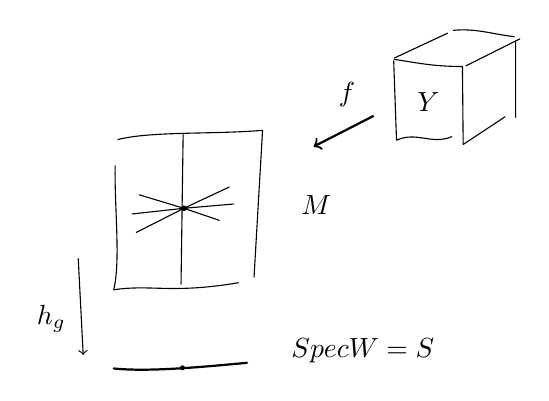
\begin{tikzpicture}[x=.009cm,y=-.009cm,line cap=round,line join=round]
\draw (554,335)--(629,300) (637,296) .. controls (669,293) and (691,301) .. (723,305);
\draw (554,337) .. controls (582,341) and (607,347) .. (650,347);
\draw (655,346)--(731,308) (725,312)--(725,419);
\draw (553,339)--(557,451) .. controls (585,438) and (606,458) .. (635,446);
\draw (650,348)--(651,457)--(710,418);
\node at (602,397) {$Y$};
\draw[->,thick] (524,417)--(440,460);
\node at (487,386) {$f$};
\draw (164,450) .. controls (211,438) and (300,443) .. (368,437)--(356,644);
\draw (160,487) .. controls (159,547) and (168,621) .. (158,662) .. controls (210,654) and (240,668) .. (334,652);
\draw (256,441)--(253,654) (194,528)--(257,547)--(307,564) (190,581)--(257,547)--(321,517) (184,555)--(257,547)--(327,541);
\fill (257,547) circle[radius=4];
\node at (444,542) {$M$};
\draw[->] (108,618)--(115,754);
\node at (70,703) {$h_{\deleted{\unsure{g}}}$};
\draw[thick] (158,773) .. controls (208,778) and (281,771) .. (346,765);
\fill (255,772) circle[radius=3.5];
\node[anchor=west] at (395,748) {$\operatorname{Spec} W=S$};
\end{tikzpicture}}
Les différentes sections de $M$ sur $S$ donneront différentes façons de relever $X_0$ en un $X$ propre et lisse sur $S$. Posant
\begingroup\makeatletter\tagsleft@true\makeatother
\[
K^{\bullet}=Rf_*(\underline{\Omega}^{\cdot}_{Y/M}) \tag*{(*)}
\]
\endgroup
on voit que pour tt telle section $g$ de $M$ sur $S$, définissant un $X^{\deleted{\unsure{(g)|g|(\Sigma)}}}_g$, et
\[
f^{\deleted{\unsure{(g)|g|(\Sigma)}}}_g : X^{\deleted{(\Sigma)}}_g \longrightarrow S
\]
% slanted
\margin{$\substack{\unsure{=}\\ (k\unsure{+|-}\frac{1}{2})\log(k+1)\\ =-(k-\frac{1}{2})\unsure{\mathrm{lo}|\log}}$}
on a
\[
\mathbb{R}f_{g*}(\underline{\Omega}^{*}_{X_g/S})
\xleftarrow[\substack{\text{isom}\\\text{can}}]{\sim} g^*(K^{\cdot})
\]
($g^*$ au sens des catégories dérivées .... ). Il s'ensuit, du moins modulo torsion, que
\[
\mathbb{R}^{i} f_{g*}(\underline{\Omega}^{*}_{X_g/S})
\xleftarrow{\sim}g^{*}(\mathscr{H}^{i})
\]
% archive sheet number: 47

\scanpage{49}
\uline{Ainsi, on trouve que}, \inserted{\uline{posant} $(\unsure{a|*})$,} \uline{les complexes} $g^*(K^{\cdot})$, \uline{pour les différentes sections} $g$ \uline{de} $M$ \uline{sur} $S$ \uline{passant par} $t_0$, \uline{sont can. isom entre eux} \uline{(au sens des cat. dérivées)} \uline{donc les} $g^*(\mathscr H^i)$ (\uline{où} $\mathscr H^i=H^i(K^{\cdot})\inserted{=\mathbb R^{\unsure{i|j|\nu}}f_*(\Omega^{\cdot}_{Y/M})}$) \uline{sont \unsure{canoniqt|canoniqmt|canoniquement} isom entre eux}, \deleted{\unsure{pour}} \uline{mod torsion}. La donnée d'un tel système transitif d'isomorphismes peut être considéré comme une \uline{structure \unsure{bourbaquiste|bourbakiste} sur} $K^{\unsure{*|\cdot}}=\mathbb R f_*(\deleted{\unsure{Y}}\underline{\Omega}^{\cdot}_{Y/M})$ [en \uuline{le point} $t_0$, relativement à la base $S$], ou sur les $\mathscr H^i=\mathbb R^i f_*(\Omega^{\cdot}_{Y/M})$, \deleted{Une telle structure est \unsure{présente|présentée} p.ex. autrement} \inserted{d'espèce voisine à une \uline{structure de}} \uline{descente}. Une structure de \deleted{\unsure{cet|ce}} ce dernier type, \inserted{pour un Module $\underline E$ disons,} : supposons qu'elles sont effectives, i.e. définissent un isom
\[
\underline E\deleted{\mathscr H^{\unsure{i}}}\simeq h^{\unsure{+|*}}(\underline E_0)
\]
($\underline E_0$ un Module sur $S$], définit \unsure{un|une}
% archive sheet number: 48

\scanpage{50}
tel système transitif d'isomorphismes entre les $g^*(\underline E)$. Nous allons décrire une structure, \inserted{un peu} moins forte que celle de descente, qui définit encore un tel syst. transitif d'isom : la \uline{structure de stratification} \uline{sur $E$}, \uline{relativement à} $S$.

2. Définition générale d'une stratification. \inserted{Relations avec connexions.}

3. Système transitif d'isom qu'elle fournit, si on est sur un anneau local complet.

4. \unsure{Là|La} \deleted{idée de} connexion de Gauss-Manin.
% archive sheet number: 49

\scanpage{51}
Dans le cas où $k$ est de car. $0$, \unsure{celà|cel|ceci|cela} est donc une connexion intégrable absolue sur $\mathscr H^*$. (Manin n'utilise pas ce langage géométrique). Puis, dans le cas du $H^1$, et lorsque $K$ \deleted{est} provient d'un modèle \inserted{propre} lisse, Manin montre de façon assez compliquée que $H^1(X,\Omega^{\cdot}_{X/k})$ (qui est $\subset H^1_{\mathrm{DR}}(K/k)$) est stable par les opérations $\Theta_x$

3.5. En fait, par des arguments très simples directs, \deleted{\unsure{que|qui}} reposant sur la ``formule d'homotopie'' de Cartan
\[
d i_x+i_x d=\Theta_x
\]
on peut montrer, pour un morphisme $f:X\longrightarrow S$ :

(i) Pour toute dérivation $\xi$ de $\underline O_S$ qui se remonte, \deleted{\unsure{sur $X$,|de $X$,|en $X$,}} \inserted{loc. au dessus de $S$,} en une dérivation $\bar\xi$ de $\underline O_X$ [condition tjrs satisfaite si $X$ est \deleted{\unsure{de|est}} \uline{formellt lisse sur} $S$ et \uline{affine} sur $S$] l'effet de $(\bar\xi,\xi)$ opérant sur $\deleted{\unsure{\mathscr H|R}} f_*(\Omega^{\cdot}_{X/S})$, \unsure{est|\deleted{est}} indépendant \uline{mod} \uline{homotopie} \deleted{\unsure{du}} du choix de $\bar\xi$, donc dépend seulement de $\xi$ ; donc en particulier, \inserted{si $f$ formellt lisse et affine} les $\mathscr H^i(f_*(\Omega^{\cdot}_{X/S}))=\mathbb R^i f_*(\Omega^{\cdot}_{X/S})$ sont des Modules sur lesquels les dérivations de $S$ opèrent, -- et on vérifie la loi de linéarité et de crochet, trivialement. Si $S$ lisse sur un $T$, ceci donne pour $f_*(\Omega^{\cdot}_{X/S})$ et \unsure{ts|tous|via} les $R^i f_*(\Omega^{\cdot}_{X/S})$ des conn. intégrables rel/$T$.
% archive sheet number: 50

\scanpage{52}
(ii) Par une construction reposant \unsure{ess\textsuperscript{t}|ess\textsuperscript{l}} sur le même principe, mais seulement un peu plus sophistiquée techniquement, (cf appendice), on trouve que si $f$ est lisse \unsure{qu. cpct|qu. cpt} et qu. sép., alors
\[
\mathbb R f_*(\Omega^{\cdot}_{X/S})
\]
est muni d'une \uline{connexion} \uline{absolue canonique} [au sens des catégories dérivées]. Cela ne signifie pas tt. à fait que les $\mathbb R^i f_*(\Omega^{\cdot}_{X/S})$ sont munis individuell\textsuperscript{t} des connexions absolues ; c'est pourtant vrai si $S$ de car. $0$, et $f$ propre et lisse (car alors la formation des $R^i f_*(\Omega^{\cdot}_{X/S})$ eux-mêmes commute à l'extension de la base ....) -- ou encore, bien sûr, dans le cas lisse affine envisagé en (i) .... La vérification (pour $f$ propre, lisse) que cette connexion est compatible avec la description transcendante, est en fait triviale.

\uline{Remarques} On \unsure{pourrait|peut} espérer que ces connexions canoniques proviennent en fait de \uline{stratifications} canoniques, de façon que l'on aurait une
% archive sheet number: 51

\scanpage{53}
explication ``à priori'' de l'\deleted{construction de} \inserted{invariance} affirmée par Washnitzer-Monsky. C'est bien vrai si $S$ est de car. zéro, mais malheureusement c'est faux en car $p>0$, même si on considère pour $f$ des projections structurales de \inserted{\unsure{familles|famille} de} courbes elliptiques (= schém. elliptiques) !

Il s'agit donc pour le moment d'une relation heuristique et sentimentale, entre deux idées différentes, dont les relations exactes sont \deleted{\unsure{pas}} \inserted{loin} encore \inserted{d'avoir} été bien élucidées ......

\begin{center}
\rule{.27\linewidth}{.4pt}\\[-.6ex]
\rule{.22\linewidth}{.4pt}
\end{center}

Pour résumer, on se trouve maintenant devant un puzzle, où il s'agit de reconstituer une théorie d'ensemble \deleted{tenant compte} \deleted{et} combinant

a) Une théorie cohomologique des complexes d'opérateurs différentiels, \deleted{\unsure{qui|qui ont|pi}} (notamment en vue \inserted{d'application au complexe de DR})

b) Une étude systématique des structures stratifiées, notamment \inserted{\unsure{prises|en vue} \unsure{avec applications conceptuelles|avec explication conceptuelle|recevront des explications conceptuelles} \unsure{\deleted{satisfaisantes}|satisfaisante|topologiques}} celles qui s'introduisent

c) La théorie de Washnitzer-Monsky,
% archive sheet number: 52

\scanpage{54}
\S~4 \uline{Topos stratifiant et} \uline{topos cristallin}.

4.1. Interprétation d'une stratification relative d'un Module $\underline F$ sur $X/S$. Si on a une telle stratification, alors pour tt $S$-morphisme $f:\deleted{\unsure{X}}Y\longrightarrow X$, et tt voisinage infinitésimal $Y'$ de $Y$, \inserted{(sur $S$)} \deleted{\unsure{qui qui|qui que|qui puisse}} tel que $f$ veut bien se prolonger (localmt du moins) en $f':Y'\unsure{\mathbin{-}|\longrightarrow}X$, un système \uline{transitif} d'isom entre les $f'{}^*(\underline F)$.
\diagram{\begin{tikzcd}[ampersand replacement=\&,row sep=small]
X \arrow[dd,dash] \& \deleted{\unsure{X}}Y_{\deleted{\unsure{0}}} \arrow[l,"f"'] \arrow[d,arrows={{Hooks[harpoon]}-}] \\
\& \deleted{\unsure{X}}Y'_{\deleted{\unsure{0|n}}} \arrow[ul,"f'"'] \\
S \&
\end{tikzcd}}

On peut donc dire que la \deleted{\unsure{connexion}} \inserted{donnée d'une} stratification \deleted{\unsure{est|une}} \inserted{revient à la} donnée \deleted{\unsure{canonique|un isom}} , pour tt voisinage infinitésimal $Y'$ d'un $Y\unsure{\xrightarrow{f}|\mathrel{\overset f{-}}}X$ (sur $S$), \inserted{soumis à la condition déjà énoncée (\unsure{autom\textsuperscript{t}.|autom.} si $X/S$ form\textsuperscript{t} lisse)} d'un \uline{prolongement} \deleted{\unsure{en}} de $F$ en un \uline{Module} sur $Y'$, -- avec des conditions de fonctorialité évidentes. Pour exprimer plus commodément ce point de vue, et une variante, on va introduire un site ad-hoc.
% archive sheet number: 53

\scanpage{55}
4.2. Définition du site et du topos cristallins \inserted{de $X$ sur $S$}

Définition du site et du topos stratifiant de $X$ sur $S$

C'est pareil si $X$ form\textsuperscript{t}. lisse sur $S$.

Ce sont des topos annelés

\deleted{Description d'un} \inserted{Attention, le site n'\uline{a pas en général d'objet final} !}

Ce sont des \deleted{\unsure{sites|Sit} \unsure{fais}} et topos \uline{annelés}.

Description des \deleted{\unsure{un}} faisceaux d'ensembles en termes de faisceaux habituels. Idem pour faisceaux d'anneaux, faisceaux de Modules sur faisceaux d'anneaux etc.

Faisceaux spéciaux : les hom de changement de base sont des isom.

\diagram{\begin{tikzcd}[ampersand replacement=\&,row sep=small]
\text{Faisceaux de Modules spéciaux sur site stratifiant \inserted{de $X/S$}}
\arrow[d,phantom,"\rotatebox{90}{$\simeq$}" description] \\
\text{Faisceaux de Modules à stratification sur $X/S$.}
\end{tikzcd}}

4.3. Énonçons de suite les résultats et conjectures suivants, qui seront \deleted{\unsure{étud|étudiés}} détaillés plus tard :

\uline{Th} Si $S$ de car. $0$ et $X$ lisse sur $S$, alors
\[
H^*_{\substack{\mathrm{CRIS}\deleted{\unsure{/S|X/S}}\\\text{ou }\mathrm{STRAT}}}(X/S,\underline O_X)\simeq H^*_{\mathrm{DR}}(X/S)
\]
(isom can). \deleted{et en fait $R f_*(\underline O_X)$ est \uline{spécial}, et
\[
(R f_{\unsure{*\mathrm{cris}|*}}(\underline O_X))^{\unsure{\mathrm{ord}}}\simeq\mathbb R f_*(\Omega^{\cdot}_{X/S})\quad ....
\]}
% archive sheet number: 54

\scanpage{56}
Ceci \unsure{donne|donnera} une explication

\uline{Conj.} Si $X$ loc. de \unsure{v.|t.} f. sur $\mathbb C$, alors
\[
H^*_{\substack{\deleted{\mathrm{DR}}\unsure{\mathrm{Str}|\mathrm{Strat}}\\\text{ou }\mathrm{crist.}}}(X/\mathbb C,\underline O_X)\simeq H^*(X^{\mathrm{an}},\mathbb C)
\]

N.B. La conjecture est prouvée, grâce au th, \deleted{lorsque}, et au th. de comparaison de l'exposé 1, dans le cas où $X$ est lisse sur $\mathbb C$. Donc \uline{dans le cas lisse}, \uline{au \unsure{dessus|\deleted{dans}dessus} d'une base de} car. $0$, \uline{on} \uline{trouve une description de la coh. de} D.R. \uline{sans utiliser de différentielles}.
% archive sheet number: 55

\scanpage{57}
\uline{\unsure{Laius|Laïus}}\hfill 6.12.1966
\diagram{\begin{tikzcd}[ampersand replacement=\&,row sep=small]
X \arrow[d,"f"']\\ S
\end{tikzcd}}

Soit $F$ un Module quasi-cohérent stratifié sur $X/S$. On a vu qu'il définit un module de $X_{\mathrm{strat}}$, et par là un faisceau cosimplicial \inserted{$F^{\unsure{+|*}}=C(F)$} sur $X_{\mathrm{zar}}$, par
\[
C^n(F)=F^{(n)}=\varprojlim_i F_{\Delta^n_{X/S}(i)}
\]
[peu importe laquelle des $n+1$ projections $\Delta^{\unsure{-|n}}_{X/S}(i)\longrightarrow X$ on prend pour définir l'image inverse, il y a des isom canoniques entre eux, précisément à cause de la stratification de $F$].

\unsure{On|Cela} a
\[
\boxed{H^*(X_{\mathrm{str}},F)\simeq\mathbb H^*(X_{\mathrm{zar}},\mathbb C^*(F))}
\]

On voit donc deux théories cohomologiques ; \deleted{\unsure{qui|par}} \inserted{\deleted{dont}} \deleted{aucune ne semble \unsure{pas|devoir} à première vue} \deleted{semblent assez \unsure{distinctes} \unsure{qu'il|gén\textsuperscript{t}} \unsure{ne} pas contenir l'autre} :

a) Pour un $F$ quasi-cohérent sur $X$, on forme les $H^i(X_{\mathrm{zar}},F)$.

b) Si $F$ est \uline{stratifié}, on forme les $H^i(X_{\mathrm{strat}},F)$, qui s'explicitent par la formule plus haut.

À première vue, le lien entre ces deux théories cohomologiques semble donné exclusivement par
% archive sheet number: 56

\scanpage{58}
la formule ci-dessus ; \deleted{Il ne semble \unsure{pas|plus|donc} \unsure{pourtant|possible} que} \inserted{A priori}, la cohomologie stratifiante d'un Module stratifié s'explicite comme une hypercohomologie zariskienne (et encore, dans un complexe dont les \deleted{\unsure{op}} \unsure{différentielles|différentielle} \unsure{n'est|ne sont} pas \unsure{linéaire|linéaires} !), \deleted{et} mais l'inverse ne semble \reversemarginpar\margin{\hfill\raisebox{-10\baselineskip}[0pt][0pt]{\rule{.4pt}{10\baselineskip}}}\normalmarginpar pas vrai. On va voir pourtant que, dans un certain sens, il en est bien ainsi. À peu de choses près, on associe à tt Module quasi-cohérent $F$ (\uline{sans stratification}) un Module \deleted{quasi-cohérent} \inserted{(plutôt, un pro-Module pro-quasi-cohérent)} $Q^{\unsure{\circ|0|\cdot}}(\deleted{\unsure{M}}F)$ stratifié, dont la cohomologie stratifiante est la coh. zariskienne \uline{ordinaire} de $X$. De plus, $Q^\circ(F)$ est un foncteur en $F$, non seulement pour des hom linéaires $F\to G$, mais même \deleted{\unsure{pour un|par des}} \inserted{\unsure{(comme|(cohomo|(conoyaux}} faisceau \deleted{\unsure{additif, au sens de|distributif,|additifs, \illegible{2}}} de $\underline O_X$-modules) pour des \deleted{\unsure{hom}} \inserted{$D$} : $F\mathbin{-}G$ qui sont seulement des op. diff. rel/$S$. \deleted{\unsure{Il faut|En fait} \illegible{3}} \inserted{[-- Dans le cas très} particulier où $\operatorname{diag}_{X/S}:X\longrightarrow X\mathbin{\times}_S X$ est une immersion nilpotente, donc \deleted{\unsure{on a|au} $Q^\circ($} stratification /$S$ = donnée de descente à $S$, $Q^\circ(F)=f^*f_*(F)$].

L'intérêt \inserted{de ces diverses \unsure{vues|voies|voisins},} c'est que l'\uline{hypercoh} \inserted{\uline{zariskienne ordinaire}} \uline{d'un complexe d'op. diff peut s'interpréter comme la coh. stratifiante} \uline{du complexe} correspondant de faisceaux stratifiés ... !
% archive sheet number: 57

\scanpage{59}
les \uline{op. diff.} de $M$ dans $N$ (rel à $S$),

Alors on trouve encore un foncteur \deleted{\unsure{les|des}} \unsure{de|en} $M$, mais \deleted{\unsure{ici|(si $i$}} non à valeurs ds les $P^i$-Modules, mais \inserted{(si $i\geq1$)} seulement ds les $P^{i-1}$-Modules, où on a considéré $P^i[M]$ comme $P^{i-1}$-Module par \uline{restriction des scalaires} à l'aide de $\alpha^{i-1}:P^{i-1}\longrightarrow P^i$. \inserted{On le note alors $Q^{i-1}[M]$ $\circledast$} En particulier, $\deleted{P}Q^0[M]$ est \deleted{\unsure{de|est}} un foncteur, en $M\in\operatorname{Ob}\operatorname{Mod}(.X/S)$ \inserted{[Modules sur $\underline O_X$, avec comme hom les op. diff. \deleted{d'ordre} rel. à $S$]}, à valeurs ds les pro-$\underline O_X$-Modules.
% margin note written sideways
\margin{et qu'on utilise comme morphismes \unsure{de|des} \deleted{\unsure{objets|Modules}} \unsure{$\mathbb N$-pro-objets|N-pro-objets} ceux de Artin--Riesz, \unsure{Supposant|exprimant} qu'on ne considère que des op. diff de degré borné, ce qui est autom. si $X$ qu. cpct].}

\deleted{[$P^0[M]=M$ \deleted{est} doit être considéré comme foncteur à valeurs ds $\mathrm{Ab}(X)$].}

Notons que l'hom $\alpha^{\cdot}:P^{\unsure{*|1}}\mathbin{-}(SP)^*=Q^*$ permet de considérer $Q^*$ comme \deleted{\unsure{module}} \inserted{algèbre} \deleted{\unsure{sur}} cosimplicial sur l'\unsure{anneau} \deleted{\unsure{semi|déplacement}}cosimplicial $P^*$, et que les opérations extérieures droites
\[
\boxed{\circledast\quad Q^{i-1}[M]=P^i\otimes_{\underline O_X} M}
\]
% archive sheet number: 58

\scanpage{60}
\S~1 Coh. de De Rham ordinaire

\S~2 Tour d'horizon sur Coh. $l$-adiques. Motivations pour le désir d'une coh. $p$-adique en car. $p$.

\S~3 Tapis de Washnitzer-Monsky.

\S~4 Stratifications. Relations de W.M. avec connexions de Gauss-Manin sur coh. de De Rham

\S~5 \deleted{\unsure{Le}} Site cristallin et site stratifiant. Énoncé \deleted{de} d'un théorème et d'une conjecture en car. nulle.

\S~6 Calculs Čechistes. (car. quelconque).

\S~7 Comparaison de la Coh. de De Rham et cristalline (car. nulle).

\S~8 \deleted{\unsure{Considérations|Comparaison}} \inserted{Retour} sur le cas de la car. $p>0$

\noindent\rule{\linewidth}{.4pt}

\margin{\deleted{\uline{\unsure{Coh. topologique|Coh. stratifiée}}} \uline{Coh. stratifiante}}

6.1. Commençons à travailler sur le \deleted{\unsure{objet|site}}topos \uline{stratifiant} pour $X/S$. Il y a l'objet $\widetilde X$ de ce topos : il \uline{couvre l'objet final} (c'est ici qu'on utilise la restriction sur les objets du site stratifiant parmi ceux du site cristallin). Donc suite spectrale de Leray
\[
H^*(X_{\mathrm{Strat}},F)\Longleftarrow E^{pq}_2=H^p(\nu\rightsquigarrow H^q(\widetilde X^{\nu+1},F))
\]

Or on constate que
\[
\widetilde X^{\deleted{\unsure{p}}\nu+1}=\varinjlim_i\deleted{\unsure{\Delta_X}}\underbrace{\Delta^{(\nu)}_X(i)}_{\substack{\text{voisinage inf. $i$-ème}\\\text{de la diagonale dans}\\ X^{\nu+1}\unsure{\deleted{X'}|\longrightarrow X'}\text{, considéré comme \unsure{provoisin|provenant|provision|prosimplicial}}\\\text{de }X}}\deleted{\unsure{(X)}}
\]

D'autre part, \unsure{pour|\deleted{pour}} tt objet $(U,X')$ \deleted{\unsure{tel que}}
\diagram{\begin{tikzcd}[ampersand replacement=\&,row sep=tiny,column sep=tiny]
X \& U\arrow[l,hook']\arrow[dr]\\
\&\&X'
\end{tikzcd}}
du site stratifiant, on aura
% archive sheet number: 59

